\documentclass{article}
\usepackage[utf8]{inputenc}
\usepackage{listings}
\usepackage{multimedia} % to embed movies in the PDF file
\usepackage{graphicx}
\usepackage{comment}
\usepackage[english]{babel}
\usepackage{amsmath}
\usepackage{amsfonts}
\usepackage{wrapfig}
\usepackage{multirow}
\usepackage{verbatim}
\usepackage{float}
\usepackage{cancel}
\usepackage{caption}
\usepackage{subcaption}
\usepackage{/home/cade/Homework/latex-defs}


\title{AMATH 569 Homework 1}
\author{Cade Ballew \#2120804}
\date{April 13, 2022}

\begin{document}
	
\maketitle
	
\section{Problem 1}
We consider the IVP 
\begin{align*}
\begin{cases}
	\frac{\partial }{\partial t}u+u\frac{\partial }{\partial x}u=0\\
	u(x,0)=f(x)
\end{cases}
\end{align*}
where
\[
f(x)=\begin{cases}
	1, &x\leq0\\
	1-x, &0<x<1\\
	0, &x\geq1.
\end{cases}
\]

\subsection{Part a}
To find when then shock forms, we write the characteristic $x=\xi+tf(\xi)$ and use the condition from page 2 of lecture 2 and the bottom of page 10 in Bernard's notes that
\[
t^*=-\frac{1}{c'(u_0(\xi^*))u_{0\xi}(\xi^*)}
\]
where $\xi^*$ maximizes $|c'(u_0)u_{0\xi}|$ for $c'(u_0)u_{0\xi}<0$ for the general IVP
\begin{align*}
	\begin{cases}
		\frac{\partial }{\partial t}u+c(u)\frac{\partial }{\partial x}u=0\\
		u(x,0)=u_0(x).
	\end{cases}
\end{align*}
In our case, $c(u)=u$ and $u_0(x)=f(x)$. We can compute
\[
f'(x)=\begin{cases}
	0, &x<0,~x>1\\
	-1, &0<x<1,
\end{cases}
\]
and
\[
c'(u_0(\xi))u_{0\xi}(\xi)=f'(\xi).
\]
Combining these, $f'(\xi)<0$ only for $\xi\in(0,1)$ at which $f'(\xi)=-1$, so 
\[
t^*=-\frac{1}{-1}=1,
\]
and 
\[
x^*=\xi^*+t^*f(\xi^*)=\xi^*+(1-\xi^*)=1.
\]
Thus, our shock first forms at time $t^*=1$ and position $x^*=1$. We can also see this by drawing characteristics and observing that the curves with $x\in(0,1)$ intersect at $x^*=1$.

\subsection{Part b}
The method of characteristics gives that our solution is $u(x,t)=f(\xi)$. Using our characteristic, if $\xi\leq0$, $x=\xi+t$, so $\xi=x-t$. If $0<\xi<1$, $x=\xi+t(1-\xi)$, so $\xi=\frac{x-t}{1-t}$. If $\xi\geq1$, $x=\xi$. Thus,
\begin{align*}
u(x,t)&=\begin{cases}
	f(x-t), &x-t\leq0\\
	f\left(\frac{x-t}{1-t}\right), &0<\frac{x-t}{1-t}<1\\
	f(x), &x\geq1
\end{cases}=\begin{cases}
1, &x-t\leq0\\
1-\frac{x-t}{1-t}, &0<\frac{x-t}{1-t}<1\\
0, &x\geq1
\end{cases}\\&=
\begin{cases}
	1, &x\leq t\\
	\frac{1-x}{1-t}, &t<x<1\\
	0, &x\geq1.
\end{cases}
\end{align*}
Note that this is consistent with our observation that the shock occurs at time $t^*=1$ and position $x^*=1$. Using Desmos, we plot this solution for various $t$. For $t=0$, we observe $u$ as follows.\\
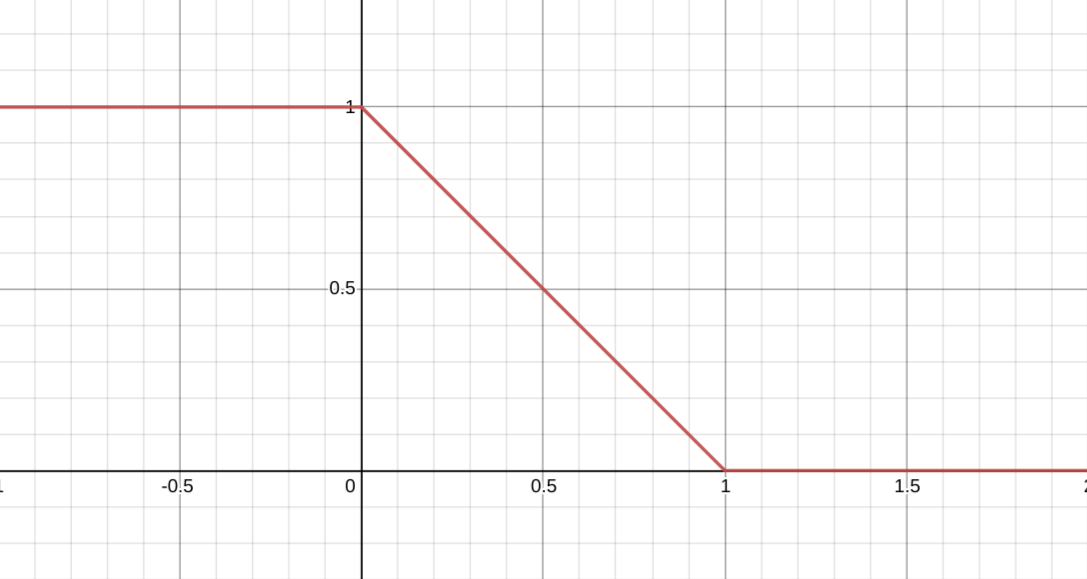
\includegraphics[scale=0.3]{graph1.png}\\
For $t=0.5$, we see \\
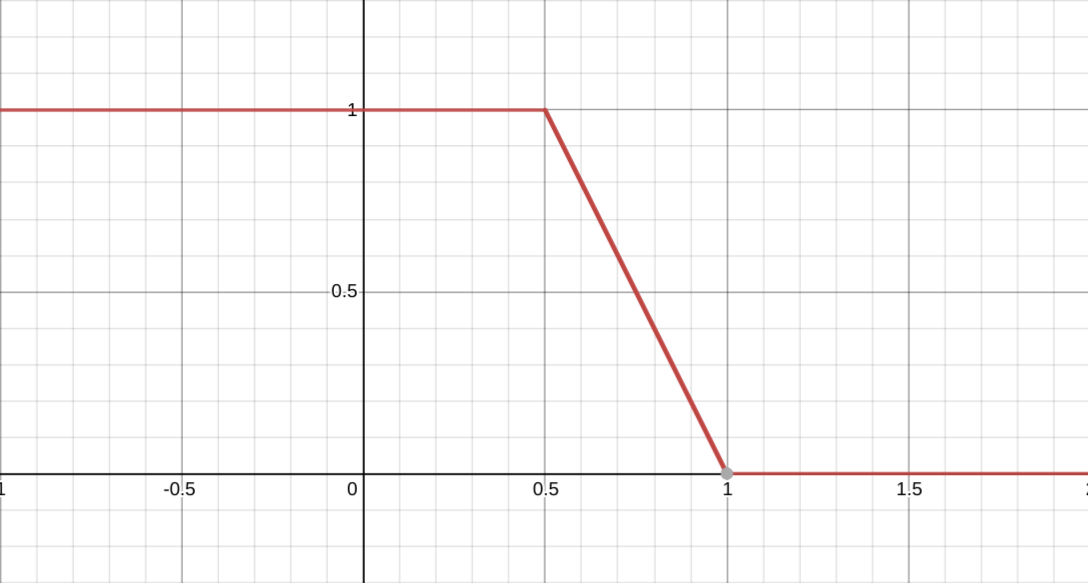
\includegraphics[scale=0.3]{graph2.png}\\
Just before the shock at $t=0.99$, we observe the following. \\
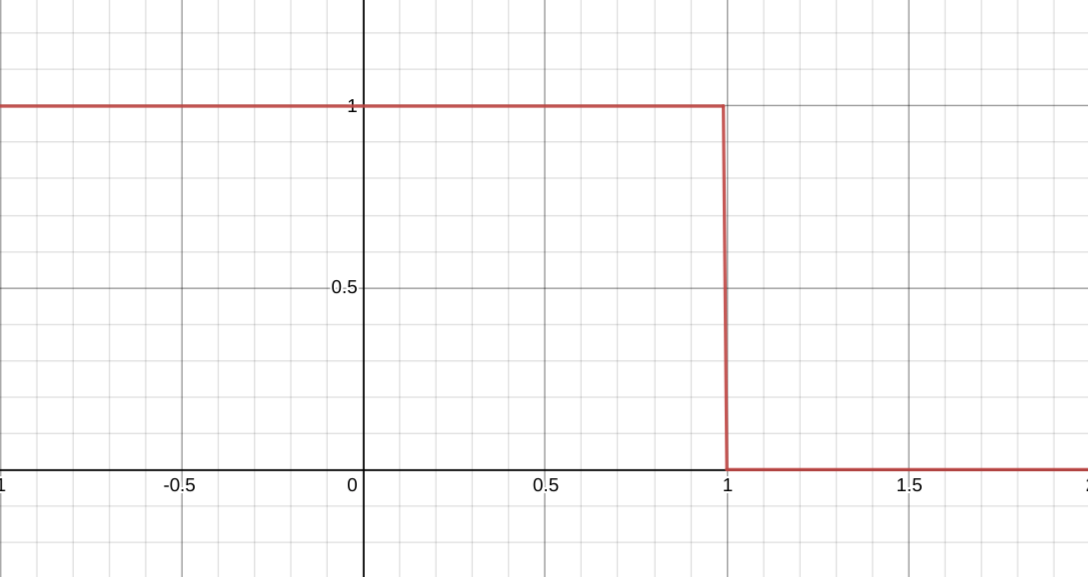
\includegraphics[scale=0.3]{graph3.png}\\

\subsection{Part c}
Note that
\[
u\frac{\partial }{\partial x}u=\frac{\partial }{\partial x}\left(\frac{1}{2}u^2\right). 
\]
Then, the Rankine-Hugoniot condition gives that the shock speed is 
\[
\dot{X}(t)=\frac{q_2-q_1}{u_2-u_1}=\frac{\frac{1}{2}u_2^2-\frac{1}{2}u_1^2}{u_2-u_1}=\frac{1}{2}(u_1+u_2)=\frac{1}{2}(1+0)=\frac{1}{2}.
\]

\subsection{Part d}
Using the shock speed, we can integrate to find that the position of the shock is $$X(t)=\frac{1}{2}t+C.$$
To determine $C$, we note that we have already found that our shock has location 1 at time 1, so $X(1)=1$, meaning that
\[
X(t)=\frac{1}{2}t+\frac{1}{2}=\frac{t+1}{2}.
\]
Knowing this, we expect that after the shock
\begin{align*}
u(x,t)=\begin{cases}
	1, &x<X(t)\\
	0, &x>X(t)
\end{cases}=\begin{cases}
1, &x<\frac{t+1}{2}\\
0, &x>\frac{t+1}{2}.
\end{cases}
\end{align*}
Plotting this with Desmos, at $t=1.01$, we get\\
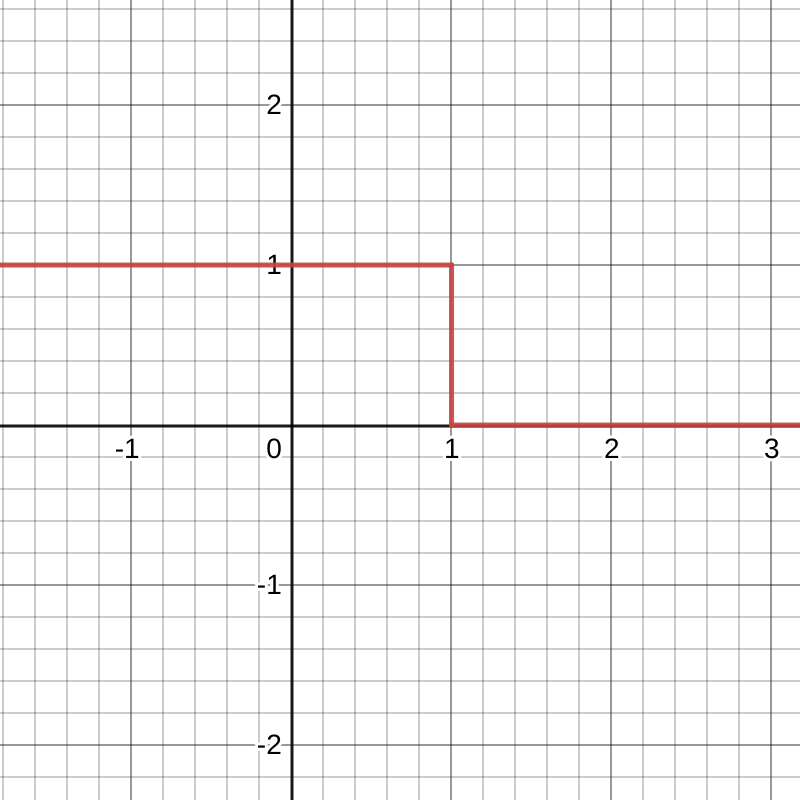
\includegraphics[scale=0.4]{graph4.png}\\
and at $t=2$, we get\\
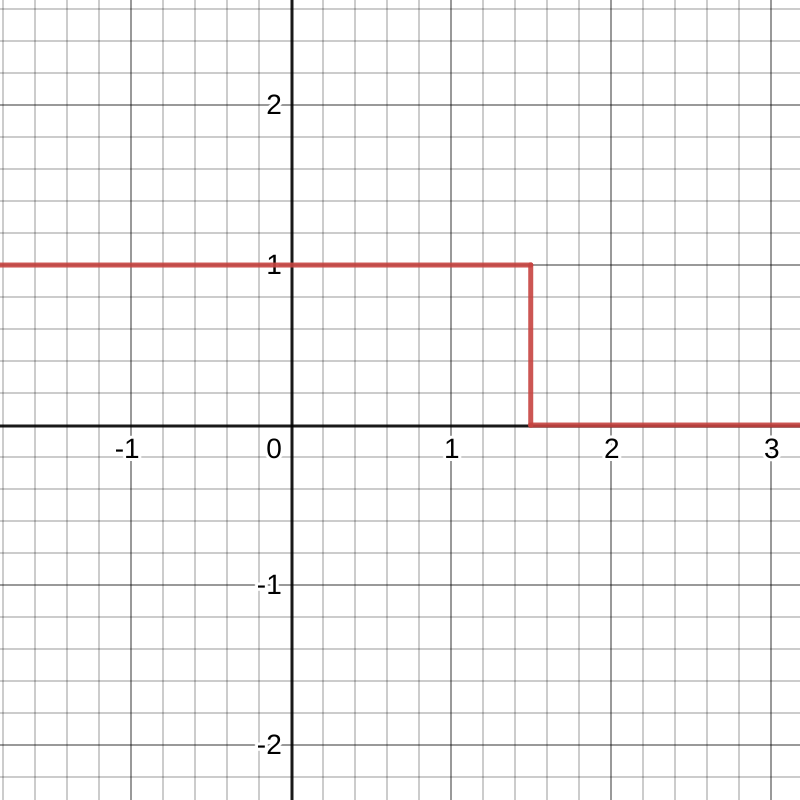
\includegraphics[scale=0.4]{graph5.png}\\

\section{Problem 2}
Now, we consider the IVP 
	\[
	\frac{\partial }{\partial t}u+u\frac{\partial }{\partial x}u= \epsilon \frac{\partial^2 }{\partial x^2}u, ~~~ - \infty < x < \infty, ~ t > 0,
\]
Subject to the initial condition
\[
u(x,0) =u_0(x)= \begin{cases}
	- 1 & x < 0 \\
	1 & x > 0 
\end{cases}
\]
where $0<\epsilon<1$. To find the outer solution, we set $\epsilon\to0$ and keep all the terms $\OO(1)$. Namely, we solve the IVP
\[
\frac{\partial }{\partial t}u+u\frac{\partial }{\partial x}u= 0, ~~~ - \infty < x < \infty, ~ t > 0,
\]
with the same initial condition. Since this does not have a value at $x=0$, we set $u_0(0)=c\in[-1,1]$. Using the method of characteristics,
\[
x=\xi+tu_0(\xi).
\]
If $\xi<0$, $x=\xi-t$, so $\xi=x+t$. If $\xi>0$, $x=\xi+t$, so $\xi=x-t$. If $\xi=0$, $x=ct$, so $c=x/t$. Note that this implies that $-1\leq \frac{x}{t}\leq1$. Thus, the outer solution is given by
\begin{align*}
u^0(x,t)=
\begin{cases}
	u_0(x+t), &x+t<0\\
	u_0(0), &-1\leq \frac{x}{t}\leq1\\
	u_0(x-t), &x-t>0
\end{cases}=
\begin{cases}
	-1, &x<-t\\
	\frac{x}{t}, &-t\leq x\leq t\\
	1, &x>t.
\end{cases}
\end{align*} 

\section{Problem 3}
Now, we instead consider the IVP 
	\[
\frac{\partial }{\partial t}u+u\frac{\partial }{\partial x}u= \epsilon \frac{\partial^2 }{\partial x^2}u, ~~~ - \infty < x < \infty, ~ t > 0,
\]
Subject to the initial condition
\[
u(x,0) =u_0(x)= \begin{cases}
	1 & x < 0 \\
	-1 & x > 0 
\end{cases}
\]
where $0<\epsilon<1$.

\subsection{Part a}
To find the outer solution, we again set $\epsilon\to0$ and keep all the terms $\OO(1)$. Namely, we solve the IVP
\[
\frac{\partial }{\partial t}u+u\frac{\partial }{\partial x}u= 0, ~~~ - \infty < x < \infty, ~ t > 0,
\]
with the same initial condition. Using the method of characteristics,
\[
x=\xi+tu_0(\xi).
\]
If $\xi<0$, $x=\xi-t$, so $\xi=x+t$. If $\xi>0$, $x=\xi-t$, so $\xi=x+t$. Thus, the outer solution is given by
\[
u^0(x,t)=
\begin{cases}
	u_0(x-t), &x-t<0\\
	u_0(x+t), &x+t>0
\end{cases}=
\begin{cases}
	1, &x<t\\
	-1, &x>-t.
\end{cases}
\]
From this solution, it is clear that we have a shock when the two piecewise components of our solutions overlap, i.e., our characteristics cross when $-t<x<t$. Thus, our solution is valid in the region
\[
\{(x,t):|x|> t\}.
\]
One can also see this by plotting the characteristics and observing that this region is where they cross. 

\subsection{Part b}
Let $U=\dot{X}(t)$ be the shock speed. We let
\[
\hat{x}= x-\int_0^t Udt.
\]
Then, 
\[
u_t=\hat{x}_tu_{\hat{x}}=-Uu_{\hat{x}},
\]
and 
\[
u_x=\hat{x}_xu_{\hat{x}}=u_{\hat{x}},
\]
so 
\[
u_{xx}=(u_{\hat{x}})_x=\hat{x}_xu_{\hat{x}\hat{x}}=u_{\hat{x}\hat{x}}.
\]
Then, our equation becomes
\[
(u-U)u_{\hat{x}}=\epsilon u_{\hat{x}\hat{x}}.
\]
If we scale $\bar{x}=\frac{\hat{x}}{\delta}$, then 
\[
(u-U)u_{\bar{x}}\frac{1}{\delta}=\frac{\epsilon}{\delta^2} u_{\bar{x}\bar{x}}
\]
which can be rewritten as 
\[
(u-U)u_{\bar{x}}=\frac{\epsilon}{\delta} u_{\bar{x}\bar{x}},
\]
so we balance by taking $\delta=\epsilon$ and get that the inner equation is given by
\[
(u-U)u_{\bar{x}}=u_{\bar{x}\bar{x}}.
\]

\subsection{Part c}
We solve this equation by first integrating with respect to $\bar{x}$ to get that 
\[
\frac{1}{2}u^2-Uu+C_1=u_{\bar{x}}.
\]
To match the outer solution, we need that $u\to u^{0-}$ as $\bar{x}\to-\infty$ and $u\to u^{0+}$ as $\bar{x}\to\infty$. Noting that $u_{\bar{x}}\to0$ as $\bar{x}\to\pm\infty$ and that $u^{0\pm}=\mp1$, we can write equations
\begin{align*}
\begin{cases}
\frac{1}{2}1^2-U\cdot1+C_1=0\\
\frac{1}{2}(-1)^2-U\cdot(-1)+C_1=0
\end{cases}
\end{align*}
which become the linear system
\begin{align*}
	\begin{cases}
		-U+C_1=-\frac{1}{2}\\
		U+C_1=-\frac{1}{2}
	\end{cases}
\end{align*}
which has solution\footnote{Note that $U$ matches the Rankine-Hugoniot condition that we found previously $\dot{X}(t)=\frac{1}{2}(u^{0+}+u^{0-})=0$.} $U=0$ and $C_1=-\frac{1}{2}$. Now, we have differential equation
\[
\frac{1}{2}u^2-\frac{1}{2}=u_{\bar{x}}
\]
which is separable. We write
\[
d\bar{x}=\frac{2du}{(u-1)(u+1)}=\left(\frac{1}{u-1}-\frac{1}{u+1}\right)du.
\]
Then,
\[
\frac{u-1}{u+1}=C_2e^{\bar{x}},
\]
so 
\[
u=\frac{1+C_2e^{\bar{x}}}{1-C_2e^{\bar{x}}}.
\]
Note that $\hat{x}=x-\int_0^t Udt=x$, so $\bar{x}=x/\epsilon$, and
\[
u(x,t)=\frac{1+C_2e^{x/\epsilon}}{1-C_2e^{x/\epsilon}}.
\]
Now, we find the constant $C_2$ by enforcing that our solution be skew-symmetric as our outer solution is. In order for this to be possible for a continuous function, we need that
\[
u(0,t)=0.
\]
Enforcing this, 
$$\frac{1+C_2}{1-C_2}=0,$$
so $C_2=-1$, and 
\[
u(x,t)=\frac{1-e^{x/\epsilon}}{1+e^{x/\epsilon}}=-\tanh\left(\frac{x}{2\epsilon}\right).
\]

\end{document}
